% ============================================================
%  Computer Network Design Project – Full Documentation
%  Compile with: pdflatex -> pdflatex (two passes for TOC)
% ============================================================
\documentclass[12pt,a4paper]{report}

% --- Encoding & Language ----------------------------------------
\usepackage[utf8]{inputenc}
\usepackage[T1]{fontenc}
\usepackage[english]{babel}

% --- Page layout ------------------------------------------------
\usepackage[a4paper, top=2.5cm, bottom=2.5cm,
            left=2.5cm, right=2.5cm]{geometry}

% --- Math -------------------------------------------------------
\usepackage{amsmath}

% --- Tables -----------------------------------------------------
\usepackage{booktabs}
\usepackage{longtable}
\usepackage{array}
\usepackage{multirow}
\usepackage{makecell}
\usepackage{tabularx}

% --- Graphics ---------------------------------------------------
\usepackage{graphicx}
\usepackage{float}
\usepackage{caption}
\usepackage{pdfpages}
\usepackage{pdflscape}

% --- Colors & table row shading ---------------------------------
\usepackage[table]{xcolor}
\definecolor{rowgray}{gray}{0.93}
\definecolor{hdrblue}{RGB}{52,101,164}
\definecolor{ltblue}{RGB}{210,228,255}

% --- Header / Footer --------------------------------------------
\usepackage{fancyhdr}
\pagestyle{fancy}
\fancyhf{}
\fancyhead[L]{\small\textit{Computer Network Design Project}}
\fancyhead[R]{\small\textit{\nouppercase{\leftmark}}}
\fancyfoot[C]{\thepage}
\renewcommand{\headrulewidth}{0.4pt}
\setlength{\headheight}{15pt}

% --- Misc -------------------------------------------------------
\usepackage{setspace}
\usepackage{enumitem}
\usepackage{parskip}

% --- Hyperlinks (load last) -------------------------------------
\usepackage[colorlinks=true,
            linkcolor=blue!60!black,
            urlcolor=blue!60!black,
            citecolor=green!40!black,
            bookmarks=true,
            bookmarksopen=true,
            pdftitle={Computer Network Design Project}]{hyperref}

% --- Custom column types ----------------------------------------
\newcolumntype{L}[1]{>{\raggedright\arraybackslash}p{#1}}
\newcolumntype{C}[1]{>{\centering\arraybackslash}p{#1}}
\newcolumntype{R}[1]{>{\raggedleft\arraybackslash}p{#1}}

\newcommand{\teamleader}{Laurentiu, Grad \textnormal{(Team Leader)}}
\newcommand{\memberA}{Julien, Iancu}
\newcommand{\memberB}{Alexandru, Mihoc}
\newcommand{\memberC}{Razvan, Cosma}
\newcommand{\groupnumber}{30441}

% ================================================================
\begin{document}

% ================================================================
%  TITLE PAGE
% ================================================================
\begin{titlepage}
  \centering
  \vspace*{1.5cm}
  {\Huge\bfseries Computer Network Design Project\par}
  \vspace{0.6cm}
  {\large Two-Floor Corporate Office Building\par}
  \vspace{1.4cm}
  \rule{0.85\textwidth}{0.8pt}\\[0.8cm]
  {\large\textbf{Team Members}\par}
  \vspace{0.5cm}
  \begin{tabular}{r l}
    \toprule
    \textbf{Role} & \textbf{Name} \\
    \midrule
    Team Leader & \teamleader \\[4pt]
    Member      & \memberA \\[4pt]
    Member      & \memberB \\[4pt]
    Member      & \memberC \\[4pt]
    Group       & \groupnumber \\
    \bottomrule
  \end{tabular}
  \vspace{1.2cm}
  \rule{0.85\textwidth}{0.8pt}\\[1cm]
  \vfill
  {\large Academic Year 2025--2026\par}
  {\normalsize \today\par}
\end{titlepage}

% ================================================================
%  TABLE OF CONTENTS / LOT / LOF
% ================================================================
\tableofcontents
\listoftables
\listoffigures

% ================================================================
%  CHAPTER 1 – WIRING
% ================================================================
\chapter{Wiring}

The building is a two-floor corporate office complex, where the \textbf{ground floor} is served by two distribution frames:
the \textbf{Main Distribution Frame (MDF)} and
\textbf{Intermediate Distribution Frame IDF1}.
The \textbf{first floor} is served by \textbf{IDF2} and \textbf{IDF3}.
Rooms are numbered with the floor prefix: \texttt{1.x} for the ground
floor and \texttt{2.x} for the first floor.
Bathrooms and utility rooms (1.3, 1.9, 1.10, 1.20, 1.21, 1.28, 1.34, 1.35 and their first-floor counterparts) are excluded
from network cabling.

Room types used throughout the document are defined in
Table~\ref{tab:room_types}.

\begin{table}[H]
  \centering
  \caption{Room Type Definitions}
  \label{tab:room_types}
  \begin{tabular}{C{1cm} L{4cm} C{2cm} C{2.5cm}}
    \toprule
    \textbf{Type} & \textbf{Description} & \textbf{Area (m\textsuperscript{2})} & \textbf{Dimensions (m)} \\
    \midrule
    A & Standard Office        & 55.25  & $6.5 \times 8.5$ \\
    \rowcolor{rowgray}
    B & Reception / Lobby      & 55.25  & $8.5 \times 6.5$ \\
    C & Individual Office      & 46.75  & $5.5 \times 8.5$ \\
    \rowcolor{rowgray}
    D & Large Conference Room  & 97.75  & $8.5 \times 11.5$ \\
    E & Department Office      & 74.75  & $6.5 \times 11.5$ \\
    \rowcolor{rowgray}
    F & Open-Plan Office Space & 330.00 & $20 \times 16.5$ \\
    G & Large Meeting Room     & 200.00 & $10 \times 20$ \\
    \rowcolor{rowgray}
    H & Computer Lab           & 90.00  & $9 \times 10$ \\
    I & Seminar Room           & 58.50  & $6.5 \times 9$ \\
    \rowcolor{rowgray}
    J & Small Office           & 42.75  & $4.5 \times 9.5$ \\
    K & Collaborative Office   & 68.75  & $5.5 \times 12.5$ \\
    \rowcolor{rowgray}
    L & Multi-Purpose Room     & 70.00  & $5 \times 14$ \\
    \bottomrule
  \end{tabular}
\end{table}

% ----------------------------------------------------------------
\section{Double Outlets}
% ----------------------------------------------------------------

\subsection{Calculation Methodology}

Double RJ-45 Cat\,6 outlets are installed in every networked room.
The minimum density follows the standard of \textbf{one double outlet
per 10\,m\textsuperscript{2}} of usable floor area, rounded up,
with a minimum of one double outlet per planned workstation position.

Each double outlet provides \textbf{two simple (single) RJ-45 sockets}.

\begin{equation}
  N_{\text{double}} = \left\lceil \frac{A_{\text{room}}}{10} \right\rceil,
  \qquad
  N_{\text{simple}} = 2 \times N_{\text{double}}
  \label{eq:outlets}
\end{equation}

\subsection{Explicit Calculation Example -- Room 1.1 (Type A)}

\begin{itemize}[noitemsep]
  \item \textbf{Room:} 1.1, Type A, Standard Office
  \item \textbf{Dimensions:} $6.5\,\mathrm{m} \times 8.5\,\mathrm{m}$
  \item \textbf{Floor area:} $A = 6.5 \times 8.5 = 55.25\,\mathrm{m}^2$
  \item \textbf{Distribution frame:} MDF
\end{itemize}

Applying Equation~\ref{eq:outlets}:
\begin{align*}
  N_{\text{double}} &= \left\lceil \frac{55.25}{10} \right\rceil
                     = \lceil 5.525 \rceil = \mathbf{6\;\text{double outlets}} \\[4pt]
  N_{\text{simple}} &= 2 \times 6 = \mathbf{12\;\text{simple outlets}}
\end{align*}

\subsection{Ground Floor Outlet Summary}

\begin{longtable}{C{1.2cm} C{1.3cm} R{1.7cm} R{1.7cm} C{1.6cm} C{1.8cm} C{1.8cm}}
  \caption{Ground Floor -- MDF Zone Outlets}\label{tab:outlets_mdf}\\
  \toprule
  \textbf{Room} & \textbf{Type} & \textbf{L (m)} & \textbf{W (m)}
    & \textbf{Area (m\textsuperscript{2})} & \textbf{Double} & \textbf{Simple} \\
  \midrule
  \endfirsthead
  \multicolumn{7}{c}{\small\tablename~\thetable{} \textit{(continued)}}\\
  \toprule
  \textbf{Room} & \textbf{Type} & \textbf{L (m)} & \textbf{W (m)}
    & \textbf{Area (m\textsuperscript{2})} & \textbf{Double} & \textbf{Simple} \\
  \midrule
  \endhead
  \midrule\multicolumn{7}{r}{\small\textit{Continued on next page}}\\
  \endfoot
  \bottomrule
  \endlastfoot
  1.1  & A & 6.5  & 8.5  & 55.25  & 6  & 12 \\
  \rowcolor{rowgray}
  1.2  & B & 8.5  & 6.5  & 55.25  & 6  & 12 \\
  1.4  & C & 5.5  & 8.5  & 46.75  & 5  & 10 \\
  \rowcolor{rowgray}
  1.5  & C & 5.5  & 8.5  & 46.75  & 5  & 10 \\
  1.6  & C & 5.5  & 8.5  & 46.75  & 5  & 10 \\
  \rowcolor{rowgray}
  1.7  & C & 5.5  & 8.5  & 46.75  & 5  & 10 \\
  1.8  & C & 5.5  & 8.5  & 46.75  & 5  & 10 \\
  \rowcolor{rowgray}
  1.11 & D & 8.5  & 11.5 & 97.75  & 10 & 20 \\
  1.12 & F & 20.0 & 16.5 & 330.00 & 33 & 66 \\
  \rowcolor{rowgray}
  1.13 & E & 6.5  & 11.5 & 74.75  & 8  & 16 \\
  1.14 & E & 6.5  & 11.5 & 74.75  & 8  & 16 \\
  \rowcolor{rowgray}
  1.15 & E & 6.5  & 11.5 & 74.75  & 8  & 16 \\
  1.16 & E & 6.5  & 11.5 & 74.75  & 8  & 16 \\
  \rowcolor{rowgray}
  1.17 & E & 6.5  & 11.5 & 74.75  & 8  & 16 \\
  1.22 & G & 10.0 & 20.0 & 200.00 & 20 & 40 \\
  \midrule
  \multicolumn{5}{r}{\textbf{MDF Subtotal}} & \textbf{140} & \textbf{280} \\
\end{longtable}

\begin{longtable}{C{1.2cm} C{1.3cm} R{1.7cm} R{1.7cm} C{1.6cm} C{1.8cm} C{1.8cm}}
  \caption{Ground Floor -- IDF1 Zone Outlets}\label{tab:outlets_idf1}\\
  \toprule
  \textbf{Room} & \textbf{Type} & \textbf{L (m)} & \textbf{W (m)}
    & \textbf{Area (m\textsuperscript{2})} & \textbf{Double} & \textbf{Simple} \\
  \midrule
  \endfirsthead
  \multicolumn{7}{c}{\small\tablename~\thetable{} \textit{(continued)}}\\
  \toprule
  \textbf{Room} & \textbf{Type} & \textbf{L (m)} & \textbf{W (m)}
    & \textbf{Area (m\textsuperscript{2})} & \textbf{Double} & \textbf{Simple} \\
  \midrule
  \endhead
  \midrule\multicolumn{7}{r}{\small\textit{Continued on next page}}\\
  \endfoot
  \bottomrule
  \endlastfoot
  1.18 & E & 6.5 & 11.5 & 74.75  & 8  & 16 \\
  \rowcolor{rowgray}
  1.19 & E & 6.5 & 11.5 & 74.75  & 8  & 16 \\
  1.23 & G & 10  & 20.0 & 200.00 & 20 & 40 \\
  \rowcolor{rowgray}
  1.24 & H & 9   & 10.0 & 90.00  & 9  & 18 \\
  1.25 & H & 9   & 10.0 & 90.00  & 9  & 18 \\
  \rowcolor{rowgray}
  1.26 & I & 6.5 & 9.0  & 58.50  & 6  & 12 \\
  1.27 & I & 6.5 & 9.0  & 58.50  & 6  & 12 \\
  \rowcolor{rowgray}
  1.29 & J & 4.5 & 9.5  & 42.75  & 5  & 10 \\
  1.30 & J & 4.5 & 9.5  & 42.75  & 5  & 10 \\
  \rowcolor{rowgray}
  1.31 & J & 4.5 & 9.5  & 42.75  & 5  & 10 \\
  1.32 & J & 4.5 & 9.5  & 42.75  & 5  & 10 \\
  \rowcolor{rowgray}
  1.33 & J & 4.5 & 9.5  & 42.75  & 5  & 10 \\
  1.36 & K & 5.5 & 12.5 & 68.75  & 7  & 14 \\
  \rowcolor{rowgray}
  1.37 & K & 5.5 & 12.5 & 68.75  & 7  & 14 \\
  1.38 & K & 5.5 & 12.5 & 68.75  & 7  & 14 \\
  \rowcolor{rowgray}
  1.39 & K & 5.5 & 12.5 & 68.75  & 7  & 14 \\
  1.40 & K & 5.5 & 12.5 & 68.75  & 7  & 14 \\
  \rowcolor{rowgray}
  1.41 & K & 5.5 & 12.5 & 68.75  & 7  & 14 \\
  \midrule
  \multicolumn{5}{r}{\textbf{IDF1 Subtotal}} & \textbf{133} & \textbf{266} \\
\end{longtable}

\noindent\textbf{Ground Floor Total: 273 double outlets = \underline{546 simple outlets}}

\subsection{First Floor Outlet Summary}

The first floor mirrors the ground floor in the IDF2 zone (same room types as the MDF zone).
The IDF3 zone differs slightly: no H-type computer labs, instead, a combined L-type room is present.

\begin{longtable}{C{1.2cm} C{1.3cm} R{1.7cm} R{1.7cm} C{1.6cm} C{1.8cm} C{1.8cm}}
  \caption{First Floor -- IDF2 Zone Outlets (mirrors MDF zone)}\label{tab:outlets_idf2}\\
  \toprule
  \textbf{Room} & \textbf{Type} & \textbf{L (m)} & \textbf{W (m)}
    & \textbf{Area (m\textsuperscript{2})} & \textbf{Double} & \textbf{Simple} \\
  \midrule
  \endfirsthead
  \multicolumn{7}{c}{\small\tablename~\thetable{} \textit{(continued)}}\\
  \toprule
  \textbf{Room} & \textbf{Type} & \textbf{L (m)} & \textbf{W (m)}
    & \textbf{Area (m\textsuperscript{2})} & \textbf{Double} & \textbf{Simple} \\
  \midrule
  \endhead
  \bottomrule
  \endlastfoot
  2.1  & A & 6.5  & 8.5  & 55.25  & 6  & 12 \\
  \rowcolor{rowgray}
  2.2  & B & 8.5  & 6.5  & 55.25  & 6  & 12 \\
  2.4  & C & 5.5  & 8.5  & 46.75  & 5  & 10 \\
  \rowcolor{rowgray}
  2.5  & C & 5.5  & 8.5  & 46.75  & 5  & 10 \\
  2.6  & C & 5.5  & 8.5  & 46.75  & 5  & 10 \\
  \rowcolor{rowgray}
  2.7  & C & 5.5  & 8.5  & 46.75  & 5  & 10 \\
  2.8  & C & 5.5  & 8.5  & 46.75  & 5  & 10 \\
  \rowcolor{rowgray}
  2.11 & D & 8.5  & 11.5 & 97.75  & 10 & 20 \\
  2.12 & F & 20.0 & 16.5 & 330.00 & 33 & 66 \\
  \rowcolor{rowgray}
  2.13 & E & 6.5  & 11.5 & 74.75  & 8  & 16 \\
  2.14 & E & 6.5  & 11.5 & 74.75  & 8  & 16 \\
  \rowcolor{rowgray}
  2.15 & E & 6.5  & 11.5 & 74.75  & 8  & 16 \\
  2.16 & E & 6.5  & 11.5 & 74.75  & 8  & 16 \\
  \rowcolor{rowgray}
  2.17 & E & 6.5  & 11.5 & 74.75  & 8  & 16 \\
  2.22 & G & 10.0 & 20.0 & 200.00 & 20 & 40 \\
  \midrule
  \multicolumn{5}{r}{\textbf{IDF2 Subtotal}} & \textbf{140} & \textbf{280} \\
\end{longtable}

\begin{longtable}{C{1.2cm} C{1.3cm} R{1.7cm} R{1.7cm} C{1.6cm} C{1.8cm} C{1.8cm}}
  \caption{First Floor -- IDF3 Zone Outlets}\label{tab:outlets_idf3}\\
  \toprule
  \textbf{Room} & \textbf{Type} & \textbf{L (m)} & \textbf{W (m)}
    & \textbf{Area (m\textsuperscript{2})} & \textbf{Double} & \textbf{Simple} \\
  \midrule
  \endfirsthead
  \multicolumn{7}{c}{\small\tablename~\thetable{} \textit{(continued)}}\\
  \toprule
  \textbf{Room} & \textbf{Type} & \textbf{L (m)} & \textbf{W (m)}
    & \textbf{Area (m\textsuperscript{2})} & \textbf{Double} & \textbf{Simple} \\
  \midrule
  \endhead
  \bottomrule
  \endlastfoot
  2.18   & E & 6.5 & 11.5 & 74.75  & 8  & 16 \\
  \rowcolor{rowgray}
  2.19   & E & 6.5 & 11.5 & 74.75  & 8  & 16 \\
  2.23   & G & 10  & 20.0 & 200.00 & 20 & 40 \\
  \rowcolor{rowgray}
  2.24/25& L & 5.0 & 14.0 & 70.00  & 7  & 14 \\
  2.26   & I & 9.0 & 6.5  & 58.50  & 6  & 12 \\
  \rowcolor{rowgray}
  2.27   & I & 6.5 & 9.0  & 58.50  & 6  & 12 \\
  2.29   & J & 4.5 & 9.5  & 42.75  & 5  & 10 \\
  \rowcolor{rowgray}
  2.30   & J & 4.5 & 9.5  & 42.75  & 5  & 10 \\
  2.31   & J & 4.5 & 9.5  & 42.75  & 5  & 10 \\
  \rowcolor{rowgray}
  2.32   & J & 4.5 & 9.5  & 42.75  & 5  & 10 \\
  2.33   & J & 4.5 & 9.5  & 42.75  & 5  & 10 \\
  \rowcolor{rowgray}
  2.36   & K & 5.5 & 12.5 & 68.75  & 7  & 14 \\
  2.37   & K & 5.5 & 12.5 & 68.75  & 7  & 14 \\
  \rowcolor{rowgray}
  2.38   & K & 5.5 & 12.5 & 68.75  & 7  & 14 \\
  2.39   & K & 5.5 & 12.5 & 68.75  & 7  & 14 \\
  \rowcolor{rowgray}
  2.40   & K & 5.5 & 12.5 & 68.75  & 7  & 14 \\
  2.41   & K & 5.5 & 12.5 & 68.75  & 7  & 14 \\
  \midrule
  \multicolumn{5}{r}{\textbf{IDF3 Subtotal}} & \textbf{122} & \textbf{244} \\
\end{longtable}

\noindent\textbf{First Floor Total: 262 double outlets = \underline{524 simple outlets}}

\bigskip
\begin{table}[H]
  \centering
  \caption{Building Outlet Grand Total}
  \label{tab:outlets_total}
  \begin{tabular}{L{3cm} R{2.5cm} R{2.5cm} R{2.5cm}}
    \toprule
    \textbf{Distribution Frame} & \textbf{Double Outlets} & \textbf{Simple Outlets} & \textbf{Cable (m)} \\
    \midrule
    MDF  & 140 & 280 & 16{,}980.16 \\
    \rowcolor{rowgray}
    IDF1 & 133 & 266 & 12{,}258.04 \\
    IDF2 & 140 & 280 & 16{,}980.16 \\
    \rowcolor{rowgray}
    IDF3 & 122 & 244 & 10{,}899.02 \\
    \midrule
    \textbf{Total} & \textbf{535} & \textbf{1{,}070} & \textbf{57{,}117.38} \\
    \bottomrule
  \end{tabular}
\end{table}

% ----------------------------------------------------------------
\section{UTP Cable Quantity Calculation}
% ----------------------------------------------------------------

\subsection{Calculation Methodology}

For each room, the total UTP cable needed equals the number of simple outlets
multiplied by the cable length per outlet.
The cable length per outlet accounts for:
\begin{itemize}[noitemsep]
  \item the \textbf{horizontal distance} from the distribution frame to the room ($d_{\text{DF}}$);
  \item the \textbf{average cable span inside the room} to reach each outlet ($l_{\text{avg}}$);
  \item a \textbf{technical reserve} of 6\,m per cable (3\,m at the outlet side + 3\,m at the patch-panel side).
\end{itemize}

\begin{equation}
  L_{\text{room}} = N_{\text{simple}} \times \bigl(d_{\text{DF}} + l_{\text{avg}} + 6\bigr)
  \label{eq:utp_cable}
\end{equation}

\subsection{Detailed Example -- Room 1.1}

\begin{itemize}[noitemsep]
  \item Simple outlets: $N_{\text{simple}} = 12$
  \item Distance from room to MDF: $d_{\text{DF}} = 9.4\,\mathrm{m}$
  \item Average cable run inside room: $l_{\text{avg}} = 14\,\mathrm{m}$
  \item Technical reserve: $r = 6\,\mathrm{m}$
\end{itemize}

\[
  L_{\text{room 1.1}} = 12 \times (9.4 + 14 + 6) = 12 \times 29.4 = \mathbf{352.8\,\mathrm{m}}
\]


A summary of all rooms and their cable contributions by DF zone is
given in Table~\ref{tab:utp_by_df}.

\begin{table}[H]
  \centering
  \caption{UTP Cable Length per Room -- MDF Zone (Ground Floor)}
  \label{tab:utp_by_df}
  \begin{tabular}{C{1.2cm} C{1.3cm} R{2cm} R{2cm} R{2cm} R{2.5cm}}
    \toprule
    \textbf{Room} & \textbf{Type} & \textbf{$d_{\text{DF}}$ (m)} & \textbf{$l_{\text{avg}}$ (m)} & \textbf{Simple} & \textbf{Cable (m)} \\
    \midrule
    1.1  & A & 9.40   & 14 & 12 & 352.80 \\
    \rowcolor{rowgray}
    1.2  & B & 16.11  & 5  & 12 & 325.32 \\
    1.4  & C & 21.82  & 11 & 10 & 388.20 \\
    \rowcolor{rowgray}
    1.5  & C & 27.82  & 11 & 10 & 448.20 \\
    1.6  & C & 33.53  & 11 & 10 & 505.30 \\
    \rowcolor{rowgray}
    1.7  & C & 39.53  & 11 & 10 & 565.30 \\
    1.8  & C & 45.24  & 11 & 10 & 622.40 \\
    \rowcolor{rowgray}
    1.11 & D & 0.50   & 11 & 20 & 350.00 \\
    1.12 & F & 5.00   & 22 & 66 & 2{,}178.00 \\
    \rowcolor{rowgray}
    1.13 & E & 84.64  & 17 & 16 & 1{,}722.24 \\
    1.14 & E & 91.78  & 17 & 16 & 1{,}836.48 \\
    \rowcolor{rowgray}
    1.15 & E & 98.78  & 17 & 16 & 1{,}948.48 \\
    1.16 & E & 105.92 & 17 & 16 & 2{,}062.72 \\
    \rowcolor{rowgray}
    1.17 & E & 112.92 & 17 & 16 & 2{,}174.72 \\
    1.22 & G & 17.50  & 14 & 40 & 1{,}500.00 \\
    \midrule
    \multicolumn{4}{r}{\textbf{MDF Subtotal}} & \textbf{280} & \textbf{16{,}980.16} \\
    \bottomrule
  \end{tabular}
\end{table}

\subsection{Total UTP Cable Quantities}

The complete building cable totals are summarised in Table~\ref{tab:utp_total}.
The average calculated cable span across all links is approximately 53.4\,m,
confirming the design stays well within the Cat\,6 maximum segment length of 100\,m.

\begin{table}[H]
  \centering
  \caption{UTP Cable Total Summary}
  \label{tab:utp_total}
  \begin{tabular}{L{4cm} R{3cm}}
    \toprule
    \textbf{Parameter} & \textbf{Value} \\
    \midrule
    Total cable & 57{,}117.38\,m \\
    \rowcolor{rowgray}
    Technical reserve         & 10\% \\
    Total with reserve  & 62{,}829\,m \\
    \rowcolor{rowgray}
    Average cable span        & $\approx$ 53.4\,m \\
    \bottomrule
  \end{tabular}
\end{table}

% ----------------------------------------------------------------
\section{UTP Cable Boxes}
% ----------------------------------------------------------------

UTP Cat\,6 cable is procured in 305\,m boxes.
The number of boxes required is:

\begin{equation}
  N_{\text{boxes}} = \left\lceil \frac{L_{\text{total, with reserve}}}{305} \right\rceil
  = \left\lceil \frac{62{,}829}{305} \right\rceil
  = \lceil 205.8 \rceil = \mathbf{207\;\text{boxes}}
\end{equation}

Equivalently in 2\,km reels:

\[
  N_{\text{reels}} = \left\lceil \frac{62{,}829}{2{,}000} \right\rceil
  = \lceil 31.4 \rceil \approx \mathbf{29\;\text{reels (2\,km each)}}
\]

The two procurement options are summarised in Table~\ref{tab:utp_boxes}.

\begin{table}[H]
  \centering
  \caption{UTP Cable Procurement Options}
  \label{tab:utp_boxes}
  \begin{tabular}{L{4cm} R{2cm} R{2cm} R{2.5cm}}
    \toprule
    \textbf{Format} & \textbf{Length/unit} & \textbf{Quantity} & \textbf{Total length (m)} \\
    \midrule
    Standard box (305\,m)  & 305\,m  & 207 & 63{,}135 \\
    \rowcolor{rowgray}
    Large reel (2\,000\,m) & 2{,}000\,m & 29 & 58{,}000 \\
    \bottomrule
  \end{tabular}
\end{table}

% ----------------------------------------------------------------
\section{Fiber Optic Cable Calculation}
% ----------------------------------------------------------------

\subsection{Backbone Topology}

The four distribution frames are interconnected by OM4 multimode fiber optic (50/125\,\textmu m) in a \textbf{redundant ring/mesh topology}, providing multiple paths between any two DFs. The node labelling used in the cable-planning spreadsheet is:
\begin{itemize}[noitemsep]
  \item \textbf{A} = MDF \quad \textbf{B} = IDF1 \quad \textbf{C} = IDF2 \quad \textbf{D} = IDF3
  \item suffix \textbf{0} = primary port; suffix \textbf{1} = secondary (redundant) port
\end{itemize}

\subsection{Detailed Fiber Link Calculation}

\begin{table}[H]
  \centering
  \caption{Fiber Optic Backbone Links}
  \label{tab:fo_links}
  \begin{tabular}{C{1.5cm} C{1.5cm} R{2cm} L{6cm}}
    \toprule
    \textbf{Source} & \textbf{Target} & \textbf{Length} & \textbf{Description} \\
    \midrule
    A0 & B0 & 35 m  & MDF $\to$ IDF1, ground-floor backbone \\
    \rowcolor{rowgray}
    B1 & A1 & 85 m & IDF1 $\to$ MDF, redundant inter-floor path \\
    C0 & D0 & 35 m & IDF2 $\to$ IDF3, first-floor backbone \\
    \rowcolor{rowgray}
    D1 & C1 & 85 m & IDF3 $\to$ IDF2, redundant inter-floor path \\
    A1 & C1 & 5 m  & MDF $\leftrightarrow$ IDF2, adjacent riser cross-connect \\
    \rowcolor{rowgray}
    D0 & B0 & 5 m  & IDF3 $\leftrightarrow$ IDF1, adjacent riser cross-connect \\
    A0 & C0 & 5 m  & MDF $\leftrightarrow$ IDF2, primary riser cross-connect \\
    \rowcolor{rowgray}
    D1 & B1 & 5 m  & IDF3 $\leftrightarrow$ IDF1, primary riser cross-connect \\
    \midrule
    \multicolumn{2}{l}{\textbf{Total (raw)}} & \textbf{260 m} & \\
    \multicolumn{2}{l}{+ 15\% procurement reserve} & \textbf{299 m} & rounded to 300\,m \\
    \bottomrule
  \end{tabular}
\end{table}

\textbf{Detailed example: Link A0 $\to$ B0:}
\begin{align*}
  L_{\text{raw}}    &= 35\,\mathrm{m} \quad\text{(measured in floor plan)} \\
  L_{\text{reserve}}&= 35 \times 1.15 = 40.25\,\mathrm{m} \approx 41\,\mathrm{m}
\end{align*}

Duplex OM4 cable is used, so both transmit and receive fibers are contained in a
single cable run. The total cable procurement for the entire backbone is:

\[
  L_{\text{FO, total}} = 260\,\mathrm{m} \times 1.15 \approx \mathbf{300\,\mathrm{m}}
  \quad \text{(one 300\,m reel of duplex OM4)}
\]

Each distribution frame is equipped with one \textbf{PP-72X100G-MMF} fiber patch panel
(72 LC duplex ports, OM4 compatible), accommodating all backbone connections and future expansion.

% ================================================================
%  CHAPTER 2 – VLANs AND IP ADDRESS ASSIGNMENT
% ================================================================
\chapter{VLANs and IP Address Assignment}

\section{IP Addressing Scheme}

The network uses a \textbf{private address space} under the block \texttt{10.10.0.0/16}, NAT-ed to the public IP address \texttt{203.0.113.0}. VLANs are segmented to isolate traffic types and departments. The \textbf{Management VLAN} is protected from all other VLANs by firewall policy.

Total network capacity planning:
\begin{itemize}[noitemsep]
  \item Total workstations: 928
  \item Total IP phones: 67
  \item Total wireless clients (AP capacity): up to 1{,}000
  \item Estimated peak network traffic: \textbf{32\,Gbps}
\end{itemize}

\section{VLAN Assignment Table}

\begin{longtable}{C{1cm} L{3.2cm} C{3.2cm} C{2.2cm} C{2cm} C{1.5cm}}
  \caption{VLAN and IP Address Plan}\label{tab:vlans}\\
  \toprule
  \textbf{VLAN} & \textbf{Name} & \textbf{Network} & \textbf{Gateway} & \textbf{Mask} & \textbf{Hosts} \\
  \midrule
  \endfirsthead
  \multicolumn{6}{c}{\small\tablename~\thetable{} \textit{(continued)}}\\
  \toprule
  \textbf{VLAN} & \textbf{Name} & \textbf{Network} & \textbf{Gateway} & \textbf{Mask} & \textbf{Hosts} \\
  \midrule
  \endhead
  \midrule\multicolumn{6}{r}{\small\textit{Continued on next page}}\\
  \endfoot
  \bottomrule
  \endlastfoot
  \rowcolor{ltblue}
  10  & Management      & 10.1.10.0    & 10.1.10.1   & /24 & 254 \\
  20  & IP\_Phones      & 10.1.20.0    & 10.1.20.1   & /24 & 254 \\
  \rowcolor{rowgray}
  32  & WLESS           & 10.1.32.0    & 10.1.32.1   & /22 & 1022 \\
  40 & HR               & 10.1.40.0    & 10.1.40.1   & /24 & 254 \\
  \rowcolor{rowgray}
  50 & Finance          & 10.1.50.0    & 10.1.50.1   & /24 & 254 \\
  \midrule
  \multicolumn{5}{r}{\textbf{Total usable IP addresses}} & \textbf{1526} \\
\end{longtable}

\noindent\textbf{Management VLAN security note:}
VLAN\,10 (Management) is accessible exclusively from designated management hosts.
Access from all other VLANs to VLAN\,10 is \textbf{blocked} at the L3 switch and
enforced by ACL on the Cisco Catalyst 9410R supervisors.
Remote access to all network devices (SSH) is available only through VLAN\,10.

% ================================================================
%  CHAPTER 3 – EQUIPMENT SELECTION
% ================================================================
\chapter{Equipment Selection}

For each equipment category, two options are compared.
\textbf{Option~1 (Cisco)} was selected as the preferred choice, with a 
justification given in Section~\ref{sec:equip_justification}.

% ----------------------------------------------------------------
\section{L2/L3 Modular Switch Chassis}
% ----------------------------------------------------------------

\begin{table}[H]
  \centering
  \caption{Switch Chassis Comparison}
  \label{tab:chassis_compare}
  \begin{tabular}{L{3.8cm} L{5.2cm} L{5.2cm}}
    \toprule
    \textbf{Specification} & \textbf{Option 1: Cisco Catalyst 9410R} & \textbf{Option 2: HPE Aruba CX 6410 v2} \\
    \midrule
    Chassis slots          & 10 line-card slots              & 6 line-card slots \\
    \rowcolor{rowgray}
    Max access ports       & 480$\times$ 1\,GE or 48$\times$ mGig & 480$\times$ 1\,GE PoE \\
    Backplane              & 3.2\,Tbps                       & 1.6\,Tbps \\
    \rowcolor{rowgray}
    OS                     & Cisco IOS-XE (DNAC ready)       & AOS-CX \\
    L3 routing             & Full (OSPF, BGP, EIGRP, VRF)    & Full (OSPF, BGP) \\
    \rowcolor{rowgray}
    Redundant supervisors  & Yes (dual SUP slots)            & Yes \\
    PoE budget max         & 8$\times$3\,200\,W PSU          & 4$\times$3\,600\,W PSU \\
    \rowcolor{rowgray}
    Unit price       & \$6{,}100.82                    & \$26{,}334.70 \\
    \bottomrule
  \end{tabular}
\end{table}

% ----------------------------------------------------------------
\section{Supervisor / L3 Module}
% ----------------------------------------------------------------

\begin{table}[H]
  \centering
  \caption{Supervisor Module Comparison}
  \label{tab:sup_compare}
  \begin{tabular}{L{3.8cm} L{5.2cm} L{5.2cm}}
    \toprule
    \textbf{Specification} & \textbf{Option 1: Cisco C9400-SUP-1XL} & \textbf{Option 2: HPE CX 6400 Mgmt Module} \\
    \midrule
    Uplink ports           & 2$\times$40\,GE + 2$\times$25\,GE      & 2$\times$100\,GE QSFP28 \\
    \rowcolor{rowgray}
    Forwarding rate        & 480\,Mpps                                & 400\,Mpps \\
    Power consumption      & 350\,W                                   & 200\,W \\
    \rowcolor{rowgray}
    HA features            & In-Service Software Upgrade (ISSU)       & ISSU \\
    Management             & NetConf, RestConf, YANG                  & REST API \\
    \rowcolor{rowgray}
    Unit price       & \$7{,}123.14                             & \$14{,}125.61 \\
    \bottomrule
  \end{tabular}
\end{table}

% ----------------------------------------------------------------
\section{48-Port Access Line Card (Data / IP Phone)}
% ----------------------------------------------------------------

\begin{table}[H]
  \centering
  \caption{48-Port PoE Line Card Comparison}
  \label{tab:lc48_compare}
  \begin{tabular}{L{3.8cm} L{5.2cm} L{5.2cm}}
    \toprule
    \textbf{Specification} & \textbf{Option 1: Cisco C9400-LC-48P} & \textbf{Option 2: HPE CX 6400 R0X39C} \\
    \midrule
    Port count             & 48$\times$ 1\,GE RJ-45            & 48$\times$ 1\,GE RJ-45 \\
    \rowcolor{rowgray}
    PoE standard           & 802.3at PoE+ (30\,W/port)         & 802.3at PoE+ \\
    Max PoE budget         & 2{,}880\,W                         & 740\,W \\
    \rowcolor{rowgray}
    Throughput per card    & 96\,Gbps                           & 96\,Gbps \\
    Unit price       & \$4{,}959.83                       & \$5{,}350.00 \\
    \bottomrule
  \end{tabular}
\end{table}

% ----------------------------------------------------------------
\section{Fiber Optic Line Card (min 40Gbps ports)}
% ----------------------------------------------------------------

\begin{table}[H]
  \centering
  \caption{FO Line Card Comparison (min 40\,Gbps)}
  \label{tab:fo_lc_compare}
  \begin{tabular}{L{3.8cm} L{5.2cm} L{5.2cm}}
    \toprule
    \textbf{Specification} & \textbf{Option 1: Cisco C9400-LC-12QC} & \textbf{Option 2: HPE CX 6400 R0X45C} \\
    \midrule
    Port count             & 12$\times$ 40\,GE QSFP+           & 8$\times$ 100\,GE QSFP28 \\
    \rowcolor{rowgray}
    Min port speed         & 40\,Gbps (meets requirement)       & 100\,Gbps \\
    Total bandwidth        & 480\,Gbps                          & 800\,Gbps \\
    \rowcolor{rowgray}
    FO module (Cisco)      & QSFP-40G-SR4, \$343.64/port        & HP JL310A, \$1{,}295/port \\
    OM4 reach              & 150\,m                             & 100\,m \\
    \rowcolor{rowgray}
    Line card price  & \$17{,}336.86                      & \$47{,}650.00 \\
    \bottomrule
  \end{tabular}
\end{table}

% ----------------------------------------------------------------
\section{Multi-Gigabit AP Line Card}
% ----------------------------------------------------------------

\begin{table}[H]
  \centering
  \caption{AP Line Card Comparison}
  \label{tab:ap_lc_compare}
  \begin{tabular}{L{3.8cm} L{5.2cm} L{5.2cm}}
    \toprule
    \textbf{Specification} & \textbf{Option 1: Cisco C9400-LC-48UX} & \textbf{Option 2: HPE CX 6400 S1T83A} \\
    \midrule
    Port count             & 48$\times$ mGig (1/2.5/5/10\,GE)  & 24$\times$ 2.5\,GE SFP+ \\
    \rowcolor{rowgray}
    PoE standard           & 802.3bt PoE++ (90\,W/port)         & 802.3at PoE+ \\
    Max PoE budget         & 2{,}880\,W                         & 720\,W \\
    \rowcolor{rowgray}
    Ideal use              & WiFi 7 APs, high-density           & APs up to WiFi 6E \\
    Unit price       & \$5{,}015.78                       & \$15{,}545.00 \\
    \bottomrule
  \end{tabular}
\end{table}

% ----------------------------------------------------------------
\section{Firewall}
% ----------------------------------------------------------------

\begin{table}[H]
  \centering
  \caption{Firewall Comparison}
  \label{tab:fw_compare}
  \begin{tabular}{L{3.8cm} L{5.2cm} L{5.2cm}}
    \toprule
    \textbf{Specification} & \textbf{Option 1: Cisco Secure Firewall 4245} & \textbf{Option 2: Palo Alto PA-3440} \\
    \midrule
    FW throughput          & 70\,Gbps                             & 20\,Gbps \\
    \rowcolor{rowgray}
    IPS throughput         & 50\,Gbps                             & 12\,Gbps \\
    TLS/SSL inspection     & Yes (35\,Gbps)                       & Yes (9\,Gbps) \\
    \rowcolor{rowgray}
    Interfaces             & 2$\times$100\,GE + 16$\times$10\,GE & 4$\times$10\,GE + 12$\times$1\,GE \\
    HA support             & Active/Active, Active/Standby        & Active/Passive \\
    \rowcolor{rowgray}
    Threat intelligence    & Cisco Talos                          & PAN Threat Prevention \\
    Unit price       & \$152{,}257.81                       & \$68{,}179.32 \\
    \bottomrule
  \end{tabular}
\end{table}

% ----------------------------------------------------------------
\section{WLAN Controller}
% ----------------------------------------------------------------

\begin{table}[H]
  \centering
  \caption{WLAN Controller Comparison}
  \label{tab:wlan_ctrl_compare}
  \begin{tabular}{L{3.8cm} L{5.2cm} L{5.2cm}}
    \toprule
    \textbf{Specification} & \textbf{Option 1: Cisco CW9800L} & \textbf{Option 2: HPE Aruba Central} \\
    \midrule
    Form factor            & Physical appliance (1U)         & Cloud SaaS \\
    \rowcolor{rowgray}
    AP capacity            & 1000 APs                        & Unlimited (subscription) \\
    Throughput             & 160Gbps                         & Cloud-based \\
    \rowcolor{rowgray}
    WiFi 7 (802.11be)      & Yes                             & Yes \\
    On-premises operation  & Yes (no Internet required)      & Requires Internet \\
    \rowcolor{rowgray}
    Price model            & One-time \$3{,}686.60           & Annual subscription \\
    \bottomrule
  \end{tabular}
\end{table}

% ----------------------------------------------------------------
\section{Access Points (min IEEE 802.11be / WiFi 7)}
% ----------------------------------------------------------------

\begin{table}[H]
  \centering
  \caption{Access Point Comparison}
  \label{tab:ap_compare}
  \begin{tabular}{L{3.8cm} L{5.2cm} L{5.2cm}}
    \toprule
    \textbf{Specification} & \textbf{Option 1: Cisco CW9178I} & \textbf{Option 2: HPE Aruba AP-765} \\
    \midrule
    WiFi standard          & 802.11be (WiFi 7)                & 802.11be (WiFi 7) \\
    \rowcolor{rowgray}
    Frequency bands        & 2.4\,/\,5\,/\,6\,GHz (tri-band) & 2.4\,/\,5\,/\,6\,GHz (tri-band) \\
    Max throughput         & 6.5\,Gbps                        & 5.76\,Gbps \\
    \rowcolor{rowgray}
    MIMO streams           & 4$\times$4 (6\,GHz), 4$\times$4 (5\,GHz) & 4$\times$4 (6\,GHz) \\
    PoE requirement        & 802.3bt PoE++ (60\,W)            & 802.3bt PoE++ (30\,W) \\
    \rowcolor{rowgray}
    Uplink port            & 2.5\,GE mGig                     & 2.5\,GE mGig \\
    Unit price       & \$5{,}455.89                     & \$1{,}475.37 \\
    \bottomrule
  \end{tabular}
\end{table}

% ----------------------------------------------------------------
\section{IP Phones}
% ----------------------------------------------------------------

\begin{table}[H]
  \centering
  \caption{IP Phone Comparison}
  \label{tab:phone_compare}
  \begin{tabular}{L{3.8cm} L{5.2cm} L{5.2cm}}
    \toprule
    \textbf{Specification} & \textbf{Option 1: Cisco IP Phone 8861} & \textbf{Option 2: HP 82M93AA (HP 4110)} \\
    \midrule
    Display                & 5\,in colour VGA (800$\times$480) & 2.3\,in colour \\
    \rowcolor{rowgray}
    Wi-Fi                  & 802.11ac dual-band                & 802.11ac \\
    Bluetooth              & 4.2 (headset support)             & No \\
    \rowcolor{rowgray}
    USB                    & 2$\times$ USB (PC/charging)       & No \\
    Lines                  & 5 SIP lines                       & 2 SIP lines \\
    \rowcolor{rowgray}
    PoE standard           & 802.3at PoE+                      & 802.3af PoE \\
    Codec support          & G.711, G.722, G.729, Opus         & G.711, G.729 \\
    \rowcolor{rowgray}
    Unit price       & \$366.20                          & \$194.99 \\
    \bottomrule
  \end{tabular}
\end{table}

% ----------------------------------------------------------------
\section{Choice Justification}
\label{sec:equip_justification}
% ----------------------------------------------------------------

\subsection*{Technical Arguments for Cisco}

\begin{enumerate}[noitemsep]
  \item \textbf{Unified ecosystem:} Cisco Catalyst 9000 switches, CW9178I APs,
    CW9800L controller, and Secure Firewall 4245 are all managed from a single
    \textit{Catalyst Center} dashboard, reducing operational complexity.
    \vspace{1em}
  \item \textbf{High-availability design:} The 9410R supports dual redundant
    supervisors, per-slot power-supply redundancy, and In-Service Software Upgrade (ISSU),
    enabling zero-downtime maintenance.
      \vspace{1em}


  \item \textbf{Scalability:} The modular 9410R chassis allows future line-card
    additions without replacing the chassis investment.
          \vspace{1em}


\end{enumerate}

\subsection*{Monetary Arguments for Cisco}

The total cost for the Cisco option (excluding Firewall, UPS, and cooling) is
\textbf{\$710{,}978.24}, compared to \textbf{\$791{,}727.64} for HPE Aruba, a saving of approximately \textbf{\$80{,}749.40 (10.2\%)}.


% ================================================================
%  CHAPTER 4 – ENVIRONMENT
% ================================================================
\chapter{Environment}
\label{chap:environment}

\section{Rack Size Calculation and Choice}

\subsection{Rack Layout per Distribution Frame}

Each DF is housed in a single \textbf{44U Open-Frame Server Rack}.
The rack layout is built from the bottom (UPS) upward, with ventilation
clearance rows between heat-generating equipment groups.

\begin{table}[H]
  \centering
  \caption{MDF Rack Layout (44U total)}
  \label{tab:rack_mdf}
  \begin{tabular}{C{1.5cm} C{2.5cm} L{4.5cm} L{3cm} R{2cm}}
    \toprule
    \textbf{Space (U)} & \textbf{Position} & \textbf{Equipment} & \textbf{Model} & \textbf{Power (W)} \\
    \midrule
    1  & Top    & OF Patch Panel              & PP-72X100G-MMF     & --    \\
    \rowcolor{rowgray}
    13 &        & L2/L3 Switch Chassis        & Cisco Catalyst 9410R & --   \\
       &        & \quad Supervisor $\times$2  & C9400-SUP-1XL      & 350$\times$2 \\
    \rowcolor{rowgray}
       &        & \quad OF Line Card          & C9400-LC-12QC      & 280   \\
       &        & \quad WS LC $\times$5       & C9400-LC-48P       & 65$\times$5 \\
    \rowcolor{rowgray}
       &        & \quad IP Phone LC $\times$1 & C9400-LC-48P       & 65    \\
       &        & \quad AP LC $\times$1       & C9400-LC-48UX      & 1{,}630 \\
    \rowcolor{rowgray}
       &        & \quad Fan Tray              & C9410-FAN          & 600   \\
       &        & \quad PSU $\times$3         & PWR-C4-3200WAC     & 3{,}200$\times$3 \\
    \midrule
    14 &        & UTP Patch Panel $\times$7   & CPPKL6ATG48WBL     & --    \\
    \rowcolor{rowgray}
    2  &        & Ventilation clearance       & --                 & --    \\
    1  &        & Firewall                    & Cisco FW 4245      & 1{,}380 \\
    \rowcolor{rowgray}
    2  &        & Ventilation clearance       & --                 & --    \\
    12 & Bottom & UPS $\times$2               & APC SRT10KXLT      & --    \\
    \midrule
    \textbf{44} & \textbf{Total} & & & \\
    \bottomrule
  \end{tabular}
\end{table}

\begin{table}[H]
  \centering
  \caption{IDF1 / IDF2 / IDF3 Rack Layout (39U used of 44U)}
  \label{tab:rack_idf}
  \begin{tabular}{C{1.5cm} L{4.5cm} L{3cm} R{2cm}}
    \toprule
    \textbf{Space (U)} & \textbf{Equipment} & \textbf{Model} & \textbf{Power (W)} \\
    \midrule
    1  & OF Patch Panel                  & PP-72X100G-MMF & -- \\
    \rowcolor{rowgray}
    13 & L2/L3 Switch Chassis (same config as MDF, no Firewall) & Cisco Catalyst 9410R & -- \\
    14 & UTP Patch Panel $\times$7       & CPPKL6ATG48WBL & -- \\
    \rowcolor{rowgray}
    12 & UPS $\times$2                   & APC SRT10KXLT  & -- \\
    \midrule
    \textbf{40} & \textbf{Total used} & \multicolumn{2}{l}{5U expansion headroom} \\
    \bottomrule
  \end{tabular}
\end{table}

\subsection{Rack Options}

\begin{table}[H]
  \centering
  \caption{Rack Comparison}
  \label{tab:rack_compare}
  \begin{tabular}{L{3.8cm} L{5.2cm} L{5.2cm}}
    \toprule
    \textbf{Specification} & \textbf{Option 1: APC NetShelter SX 44U} & \textbf{Option 2: Rittal TS IT 44U} \\
    \midrule
    Height                 & 44U (2{,}033\,mm)               & 44U (2{,}055\,mm) \\
    \rowcolor{rowgray}
    Type                   & Open-frame, 4-post              & Enclosed, 4-post \\
    Load capacity          & 1{,}360\,kg                     & 1{,}500\,kg \\
    \rowcolor{rowgray}
    Rail depth             & Adjustable (480--900\,mm)       & Fixed 800/1{,}000/1{,}200\,mm \\
    Airflow                & Excellent (open frame)          & Managed (perforated doors) \\
    \rowcolor{rowgray}
    Price per unit (USD)   & $\approx$\$800                  & $\approx$\$1{,}200 \\
    \textbf{Quantity}      & \textbf{4}                      & \textbf{4} \\
    \rowcolor{rowgray}
    \textbf{Total}   & \textbf{\$3{,}200}              & \textbf{\$4{,}800} \\
    \bottomrule
  \end{tabular}
\end{table}

\textbf{Choice:} APC NetShelter SX 44U open-frame rack.
The open-frame design maximises natural airflow and reduces cooling load,
is \$400 cheaper per unit, and provides easier front-rear cable access during maintenance.

% ----------------------------------------------------------------
\section{UPS Power Calculation and Choice}
% ----------------------------------------------------------------

\subsection{Power Requirement per Distribution Frame}

The required UPS power is the sum of all powered equipment in the rack,
with a 30\% safety margin per project specification.
UPS units only supply network and server equipment; cooling units are on a
separate AC circuit.

\begin{table}[H]
  \centering
  \caption{UPS Power Calculation per DF}
  \label{tab:ups_calc}
  \begin{tabular}{L{5cm} R{2cm} R{2cm} R{2cm} R{2cm}}
    \toprule
    \textbf{Parameter} & \textbf{MDF} & \textbf{IDF1} & \textbf{IDF2} & \textbf{IDF3} \\
    \midrule
    Chassis power (W)         & 4{,}030 & 4{,}030 & 4{,}030 & 4{,}030 \\
    \rowcolor{rowgray}
    Firewall (W)              & 1{,}380 & --      & --      & -- \\
    Total heat (BTU/h)        & 17{,}013 & 13{,}553 & 13{,}553 & 13{,}553 \\
    \rowcolor{rowgray}
    Required UPS power (W)    & 11{,}115 & 9{,}600 & 9{,}600 & 9{,}600 \\
    Available UPS power (W)   & 20{,}000 & 20{,}000 & 20{,}000 & 20{,}000 \\
    \rowcolor{rowgray}
    Safety margin             & 80\%  & 108\% & 108\% & 108\% \\
    \bottomrule
  \end{tabular}
\end{table}

\noindent Two \textbf{APC SRT10KXLT} units per DF give 20\,kW available, which is 80--108\% above the required load.

\subsection{UPS Options}

\begin{table}[H]
  \centering
  \caption{UPS Comparison}
  \label{tab:ups_compare}
  \begin{tabular}{L{3.8cm} L{5.2cm} L{5.2cm}}
    \toprule
    \textbf{Specification} & \textbf{Option 1: APC SRT10KXLT} & \textbf{Option 2: Eaton 9PX 10kVA} \\
    \midrule
    Rated power            & 10{,}000\,VA / 10{,}000\,W         & 10{,}000\,VA / 9{,}000\,W \\
    \rowcolor{rowgray}
    Technology             & Online double-conversion            & Online double-conversion \\
    Form factor            & Tower / 6U rack-convertible         & 6U rack \\
    \rowcolor{rowgray}
    Transfer time          & 0\,ms (always online)               & 0\,ms \\
    Runtime (50\% load)    & $\approx$15\,min (expandable)       & $\approx$15\,min \\
    \rowcolor{rowgray}
    Management             & SNMP / Web (card option)            & Network-MS card \\
    Unit price (USD)       & $\approx$\$4{,}500                  & $\approx$\$4{,}200 \\
    \rowcolor{rowgray}
    \textbf{Qty (2/DF $\times$4 DF)} & \textbf{8} & \textbf{8} \\
    \textbf{Total (USD)}   & $\approx$\textbf{\$36{,}000}        & $\approx$\$33{,}600 \\
    \bottomrule
  \end{tabular}
\end{table}

\textbf{Choice:} APC SRT10KXLT.
Wider availability, established service network, and seamless integration
with APC EcoStruxure infrastructure management platform.
The 10\,kW rating provides a larger power buffer,
which is preferred for the MDF rack housing the firewall.

% ----------------------------------------------------------------
\section{Cooling Capacity Calculation and Choice}
% ----------------------------------------------------------------

\subsection{Heat Dissipation per Distribution Frame}

Total heat dissipated must be removed by the cooling system.
A minimum 30\% additional cooling capacity is required above the calculated maximum.

\begin{table}[H]
  \centering
  \caption{Cooling Requirement per DF}
  \label{tab:cooling_calc}
  \begin{tabular}{L{5.5cm} R{2cm} R{2cm} R{2cm} R{2cm}}
    \toprule
    \textbf{Parameter} & \textbf{MDF} & \textbf{IDF1} & \textbf{IDF2} & \textbf{IDF3} \\
    \midrule
    Total heat (BTU/h)              & 17{,}013 & 13{,}553 & 13{,}553 & 13{,}553 \\
    \rowcolor{rowgray}
    Required (+30\%) (BTU/h)        & 22{,}117 & 17{,}619 & 17{,}619 & 17{,}619 \\
    Installed cooling (BTU/h)       & 38{,}000 & 38{,}000 & 38{,}000 & 38{,}000 \\
    \rowcolor{rowgray}
    Actual safety margin            & 123\%    & 180\%    & 180\%    & 180\% \\
    AC units per DF                 & 2        & 2        & 2        & 2 \\
    \bottomrule
  \end{tabular}
\end{table}

Two \textbf{Daikin Sky Air ADEAS60A} units per DF provide 38{,}000\,BTU/h.

\subsection{Cooling Options}

\begin{table}[H]
  \centering
  \caption{Cooling Unit Comparison}
  \label{tab:cooling_compare}
  \begin{tabular}{L{3.8cm} L{5.2cm} L{5.2cm}}
    \toprule
    \textbf{Specification} & \textbf{Option 1: Daikin ADEAS60A} & \textbf{Option 2: Mitsubishi PEAD-M60JA} \\
    \midrule
    Type                   & Ducted air conditioner         & Ceiling-concealed ducted \\
    \rowcolor{rowgray}
    Cooling capacity       & 6.0\,kW / 19{,}070\,BTU/h     & 6.0\,kW / 20{,}480\,BTU/h \\
    Heating capacity       & 7.0\,kW                        & 7.0\,kW \\
    \rowcolor{rowgray}
    Energy rating          & A++ (SEER 7.4)                 & A+ (SEER 6.8) \\
    Sound level (indoor)   & 28\,dB(A)                      & 30\,dB(A) \\
    \rowcolor{rowgray}
    Refrigerant            & R-32                           & R-32 \\
    Electric input         & 1{,}600\,W (cooling)           & 1{,}700\,W (cooling) \\
    \rowcolor{rowgray}
    Unit price (USD)       & $\approx$\$3{,}500             & $\approx$\$3{,}200 \\
    \textbf{Total (8 units)} & $\approx$\textbf{\$28{,}000} & $\approx$\$25{,}600 \\
    \bottomrule
  \end{tabular}
\end{table}

\textbf{Choice:} Daikin ADEAS60A.
Higher energy efficiency reduces long-term operating costs,
quieter operation, and Daikin's VRV/VRF technology
allows centralised monitoring of all 8 units.


% ================================================================
%  CHAPTER 5 – ACTIVE EQUIPMENT LIST
% ================================================================
\chapter{Active Equipment List}

TODO 
% ================================================================
%  CHAPTER 6 – MATERIAL LIST
% ================================================================
\chapter{Material List}

TODO

% ================================================================
%  CHAPTER 7 – NETWORK DRAWINGS
% ================================================================
\chapter{Network Drawings}

% ----------------------------------------------------------------
\section{Floor Plan -- Ground Floor}
% ----------------------------------------------------------------

\begin{figure}[H]
  \centering
  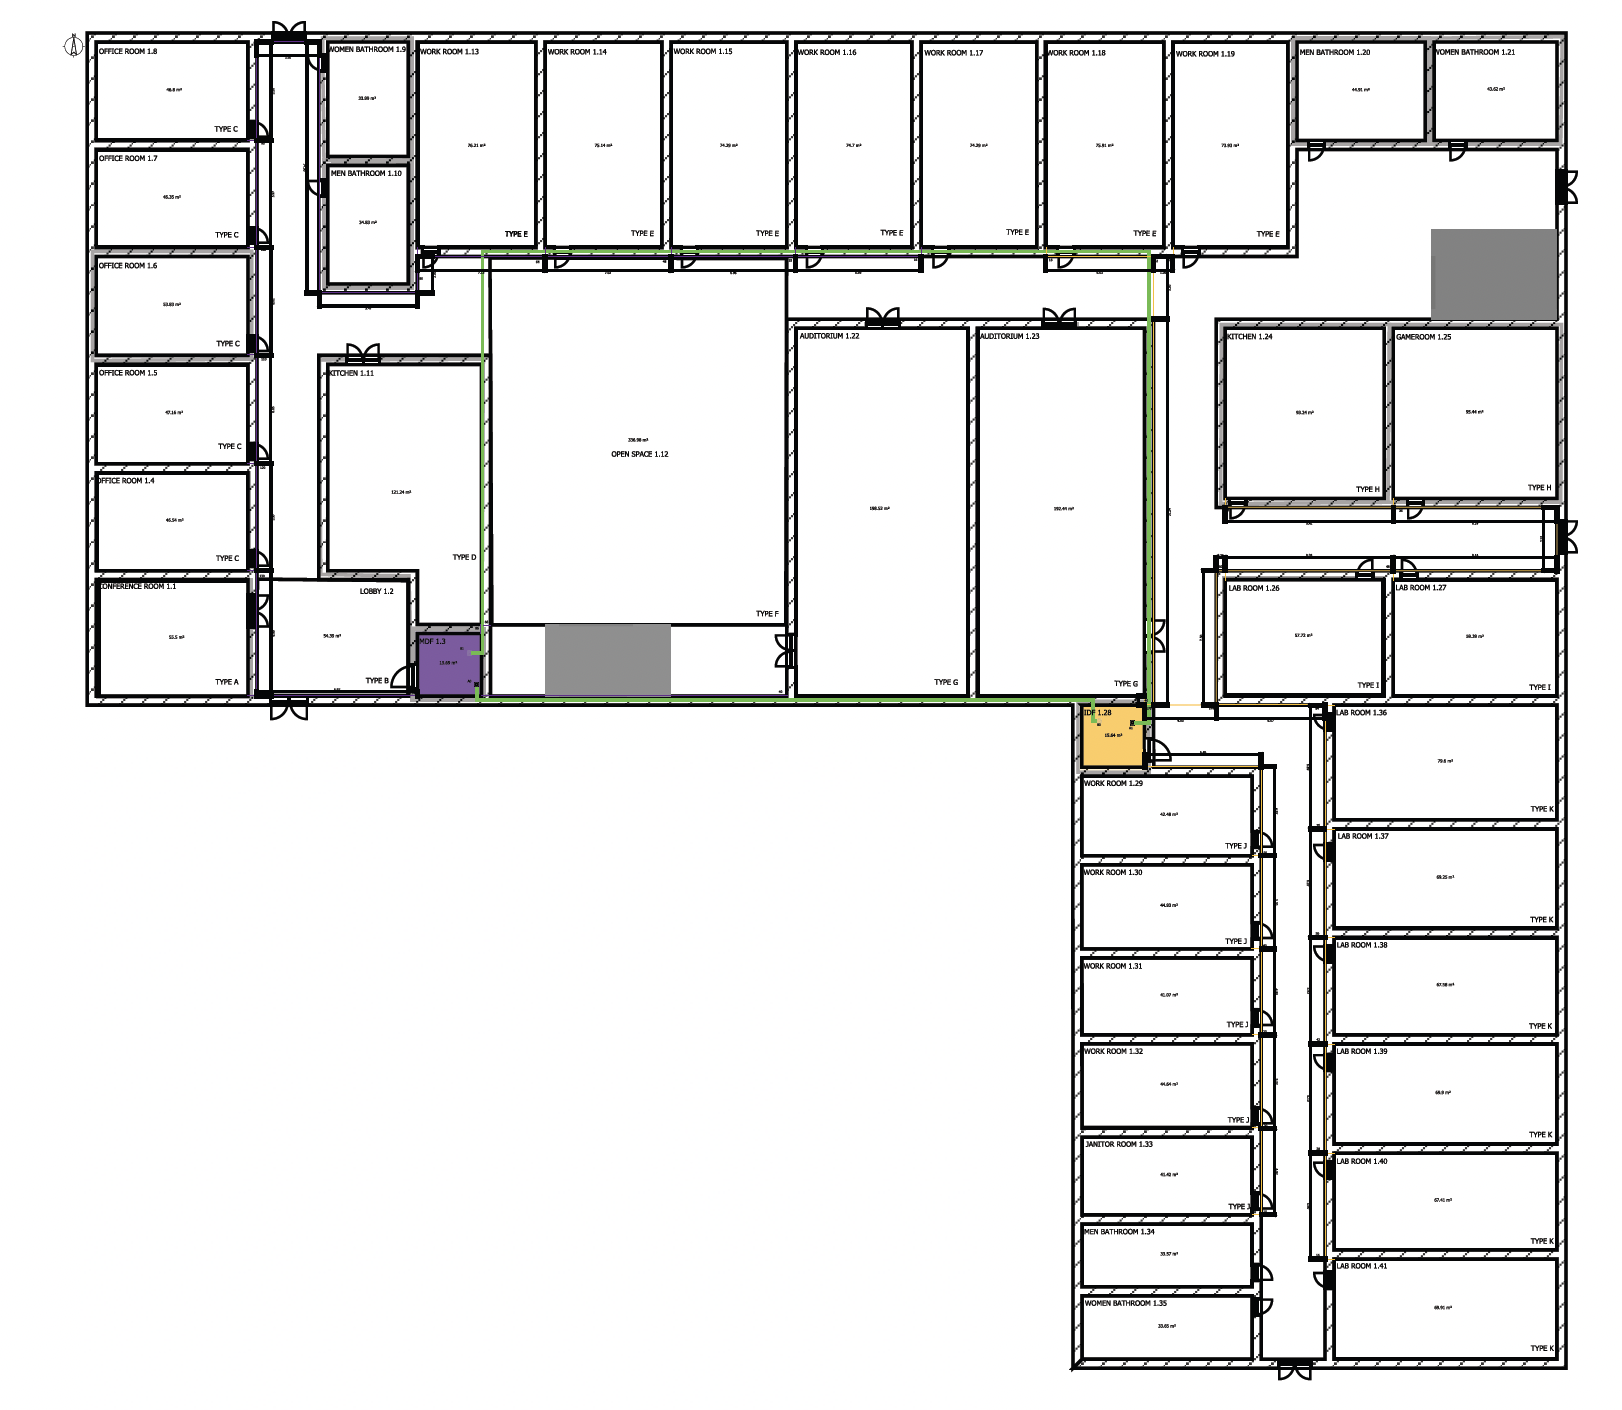
\includegraphics[width=\linewidth]{figures/ground_floor.png}
  \caption{Ground floor plan showing room layout, MDF and IDF1 locations,
           and main cable tray paths.}
  \label{fig:gf_layout}
\end{figure}

Key features:
\begin{itemize}[noitemsep]
  \item MDF room located adjacent to Room~1.11
  \item IDF1 located at the far wing, adjacent to Room~1.23
  \item Main cable tray runs along the corridor spine
  \item 22 networked rooms, bathrooms (1.3, 1.9, 1.10, 1.20, 1.21, 1.28, 1.34, 1.35) excluded
\end{itemize}

% ----------------------------------------------------------------
\section{Floor Plan -- First Floor}
% ----------------------------------------------------------------

\begin{figure}[H]
  \centering
  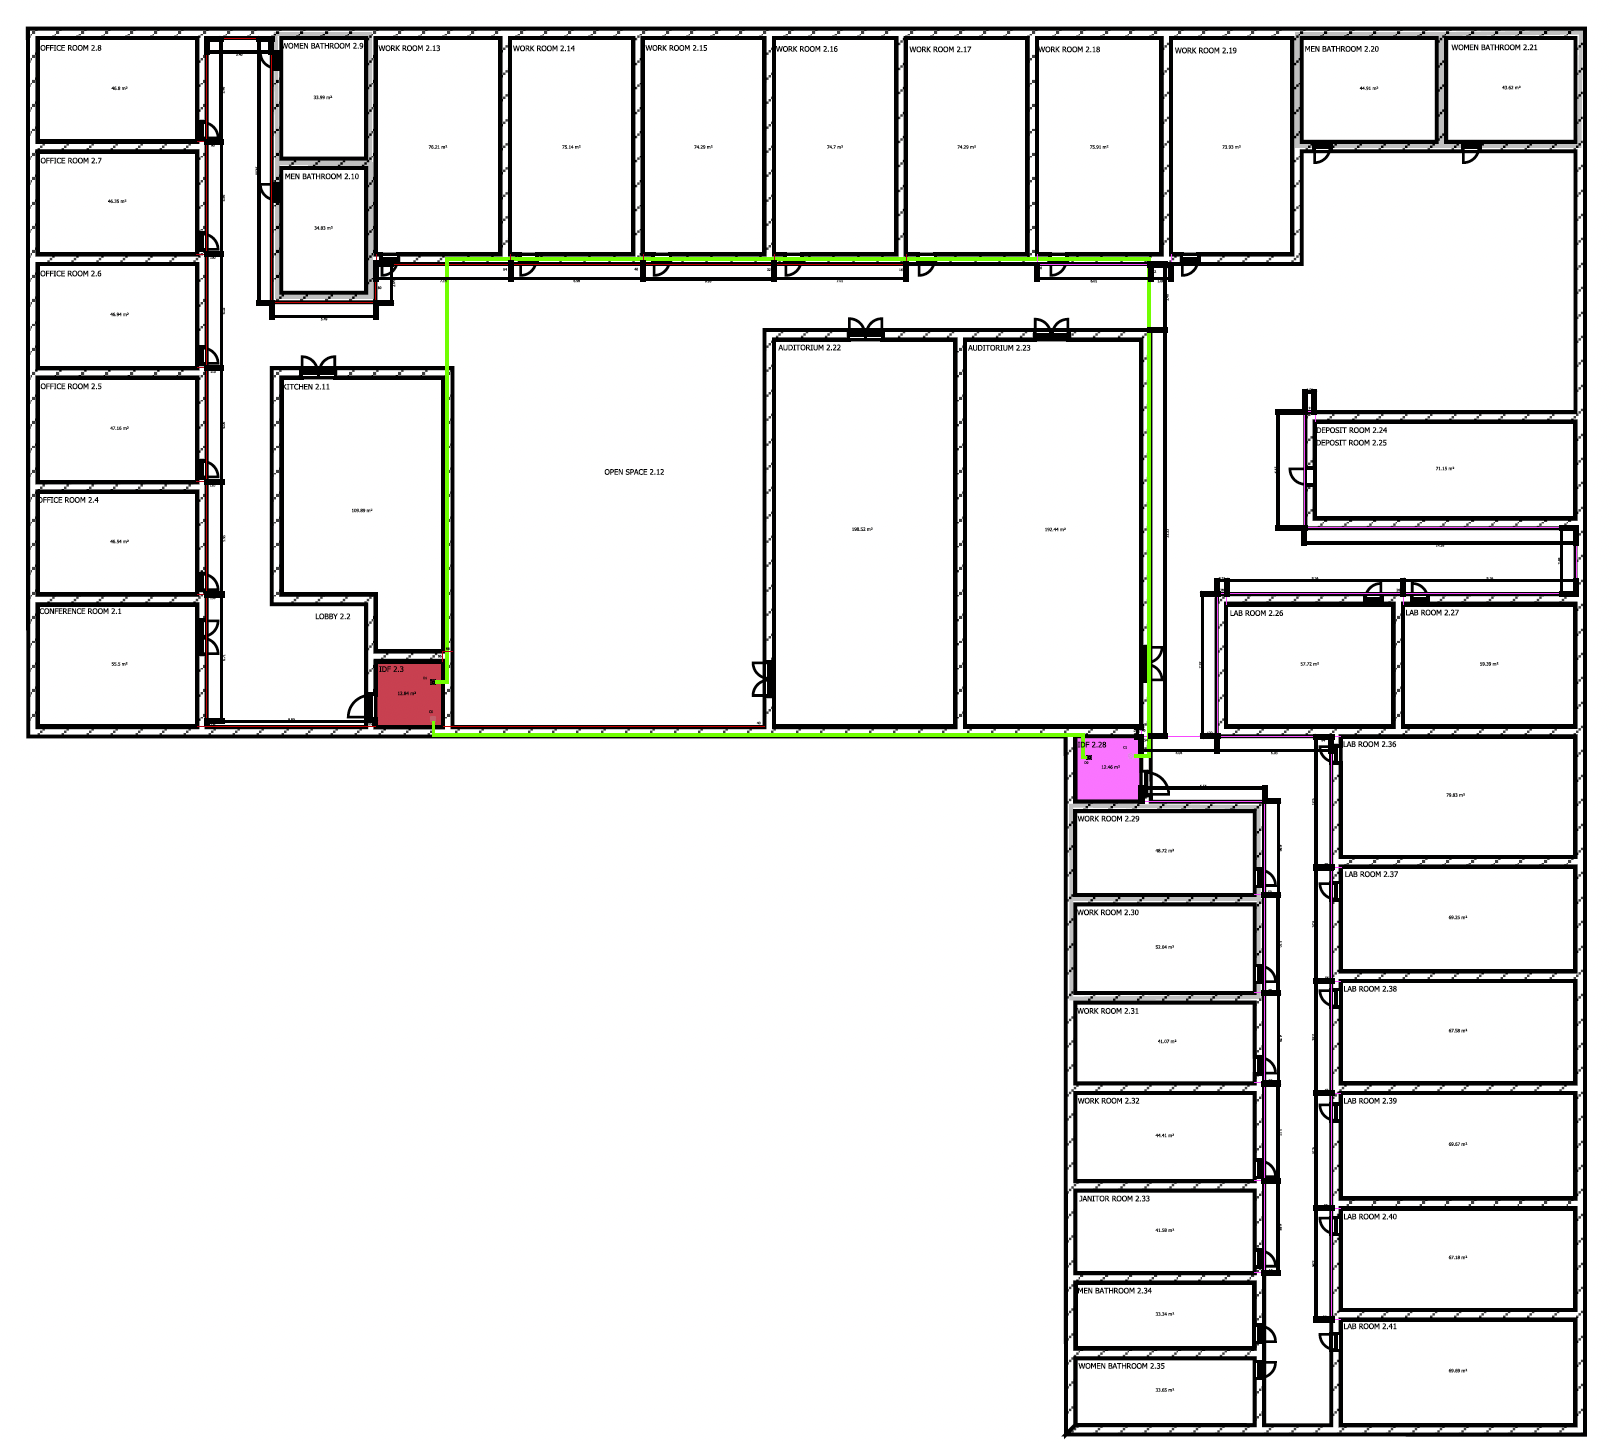
\includegraphics[width=\linewidth]{figures/first_floor.png}
  \caption{First floor plan showing room layout, IDF2 and IDF3 locations,
           and main cable tray paths.}
  \label{fig:ff_layout}
\end{figure}

Key features:
\begin{itemize}[noitemsep]
  \item IDF2 mirrors the MDF position on the floor above (adjacent to Room~2.11)
  \item IDF3 mirrors the IDF1 position on the floor above (adjacent to Room~2.23)
  \item Riser ducts in the building's vertical shaft connect floor DFs via FO backbone
  \item First floor has an additional L-type multi-purpose room (2.24/25) instead of H-type labs
\end{itemize}
\section{Cable Path Plans}

Detailed cable routing drawings with raceway paths, outlet positions,
and DF locations are provided above...

Also maybe here we can include the planning of each individual room...

\section{Network Logical Topology}

\begin{verbatim}
  Internet
     |
 [Cisco FW 4245] -- VLAN 10 (Management)
     |
 [MDF -- Cisco 9410R L3 switch / firewall uplink]
  /  |  \  \
 FO  FO  FO  FO  (40GE backbone -- ring/mesh)
 /    |    \   \
IDF1  IDF2  IDF3   (via 35m + 85m + 5m runs)
 |     |     |
L2    L2    L2   (48-port PoE line cards)
 |     |     |
WS, Phones, APs per floor zone
\end{verbatim}

\section{Rack Diagrams}

Rack layout diagrams for all four distribution frames are described in
Chapter~\ref{chap:environment} (Tables~\ref{tab:rack_mdf} and \ref{tab:rack_idf}).

TODO... maybe add something more visual

% ================================================================
%  CHAPTER 9 – REFERENCES
% ================================================================
\chapter{References}

\begin{enumerate}

  % --- Active Network Equipment ----------------------------------
  \item Cisco Catalyst 9400 Series Switch Data Sheet (covers 9410R chassis):\\
    \url{https://www.cisco.com/c/en/us/products/collateral/switches/catalyst-9400-series-switches/nb-06-cat9400-ser-data-sheet-cte-en.html}

  \item Cisco Catalyst 9400 Series -- Supervisor Engine Modules Data Sheet (C9400-SUP-1XL):\\
    \url{https://www.cisco.com/c/en/us/products/collateral/switches/catalyst-9400-series-switches/nb-06-cat9400-ser-sup-eng-data-sheet-cte-en.html}

  \item Cisco Catalyst 9400 Series -- Line Cards Data Sheet (C9400-LC-48P, C9400-LC-12QC, C9400-LC-48UX):\\
    \url{https://www.cisco.com/c/en/us/products/collateral/switches/catalyst-9400-series-switches/nb-06-cat9400-series-line-data-sheet-cte-en.html}

  \item Cisco Wireless 9178 Series Access Points Data Sheet (CW9178I -- WiFi 7):\\
    \url{https://www.cisco.com/c/en/us/products/collateral/wireless/catalyst-9100ax-access-points/wireless-9178-series-access-point-ds.html}

  \item Cisco CW9800L Wireless Controller Data Sheet:\\
    \url{https://www.cisco.com/c/en/us/products/collateral/networking/wireless/wireless-lan-controllers/cw9800l-wireless-controller-ds.html}

  \item Cisco Secure Firewall 4200 Series Data Sheet (covers 4245 model):\\
    \url{https://www.cisco.com/c/en/us/products/collateral/security/firewalls/secure-firewall-4200-ds.html}

  \item Cisco IP Phone 8861 Data Sheet:\\
    \url{https://www.cisco.com/c/en/us/products/collateral/collaboration-endpoints/unified-ip-phone-8800-series/datasheet-c78-731668.html}

  % --- Alternative Equipment (HPE / Palo Alto) -------------------
  \item HPE Aruba Networking CX 6410 v2 Switch Data Sheet:\\
    \url{https://www.hpe.com/psnow/doc/PSN1014613594WWEN}

  \item HPE Aruba Networking AP-765 WiFi 7 Access Point Data Sheet:\\
    \url{https://www.hpe.com/psnow/doc/PSN1014912441USEN}

  \item Palo Alto PA-3400 Series (PA-3440) Data Sheet -- PAN-OS 11.0:\\
    \url{https://www.paloaltonetworks.com/resources/datasheets/pa-3400-series-pan-os-11-0}

  % --- Tools -----------------------------------------------------
  \item SweetHome3D Floor Planning Tool (used for building layout):\\
    \url{https://www.sweethome3d.com/}

\end{enumerate}
\end{document}
